\documentclass{beamer}

\usepackage[utf8]{inputenc}
\usepackage[T1]{fontenc}
\usepackage[ngerman]{babel}

\usepackage{hyperref}
\usepackage{graphicx}

\usepackage[german=guillemets]{csquotes}
\usepackage{minted}

\usepackage[default,scale=0.95]{opensans}
\usepackage{fix-cm}
\usepackage{ifthen}
\usepackage{framed}

\newcommand{\LargeFact}[3][]{
	\vfill
	\begin{center}
		\ifthenelse{\equal{#1}{}}{}{\vspace{-5ex}#1\par\bigskip}
		{\fontsize{80}{80}\selectfont #2}\par
		\bigskip
		#3
	\end{center}
	\vfill
}

\title{PDF-Formulare ausfüllen mit iText \& Co.}
\subtitle{Den Papierkrieg gewinnen\ldots}
\author{Marcus Bitzl\\ \url{marcus@bitzl.com}}
\date{DANTE-Herbsttagung 	in Köln\\ 2. November 2013}

\begin{document}

%\begin{frame}{Situation: Viele Hospitationen jedes Semester}
%Jedes Semester
%\begin{itemize}
%	\item Hospitationen für 60-80 Tutoren je Semester
%	\item jeder Tutor $2\times$ (später $1-2$ mal)
%	\item Verteilt an $2-3$ Mitarbeiter
%	\item Viele Hospitationen sind auch noch parallel
%\end{itemize}
%\end{frame}

%\begin{frame}{Situation: Tutorbetrieb}
%Jedes Semester
%\begin{itemize}
%	\item {\Huge $60-80$} Tutoren je Semester
%	\item {\Huge $120-160$} Hospitation
%	\item {\Huge $2 - 10$ } Formulare je Tutoreinstellung
%	\item {\Huge $2-3$} Mitarbeiter
%\end{itemize}
%\end{frame}

\begin{frame}
	\titlepage
\end{frame}

\begin{frame}{Situation: Tutorbetrieb Informatik (TUM)}
	\LargeFact[mehr als]{80}{Tutoren jedes Semester}
\end{frame}

\begin{frame}{Situation: Tutorbetrieb Informatik (TUM)}
	\LargeFact[mehr als]{80}{Tutoren jedes Semester}
\end{frame}

\begin{frame}{Situation: Tutorbetrieb Informatik (TUM)}
	\LargeFact[ca.]{25}{Angaben je Einstellungsvorschlag}
\end{frame}

\begin{frame}{Situation: Tutorbetrieb Informatik (TUM)}
	\LargeFact[mehr als]{2000}{Angaben in den Einstellungsvorschlägen eines Semesters}
\end{frame}

\begin{frame}{Situation: Tutorbetrieb Informatik (TUM)}
	\LargeFact[mehr als]{140}{Hospitationen}
\end{frame}

\begin{frame}{Situation: Tutorbetrieb Informatik (TUM)}
	\LargeFact{2-3}{Mitarbeiter (Voll- und Teilzeit)}
\end{frame}

\begin{frame}{}
	\begin{center}
	\Huge Formulare :-)
	\end{center}
\end{frame}

%\begin{frame}{Situation: Hospitationen sind knapp}
%Dabei hat jede Hospitation
%\begin{itemize}
%\item ca 45 Minuten
%\item + \enquote{Anreise} durch das Gebäude
%\item + wenn möglich vorher mit Tutor sprechen (je nach Tutor).
%\item[$\Rightarrow$] min. 1 Stunde
%\end{itemize}
%Manchmal müssen zwei nacheinander nahtlos erfolgen, manchmal ist spontanes Umplanen nötig (z.B. Tutor krank, keine Studenten da,...).
%\end{frame}

\begin{frame}{Unsere Lösung}
Eine Webanwendung, die 
\begin{itemize}
	\item alle relevanten Informationen zum Einstellungsprozess verwaltet bzw. berechnet
	\item \ldots und damit den Einstellungsvorschlag ausfüllt
	\item alle relevanten Informationen zu den Hospitationen verwaltet
	\item \ldots und damit die Orga-Daten des Hospitationsbogens ausfüllt
\end{itemize}
\end{frame}

\begin{frame}{Unsere Lösung -- Werkzeuge}
\begin{itemize}
	\item Google Webtoolkit (GWT) für die Oberfläche
	\item Servlets für die Formulare
	\item MySQL
	\item Tomcat
\end{itemize}
\end{frame}



\begin{frame}{Verworfen: TeX generieren und PDF erzeugen}
Der Hospitationsbogen stammt von uns, den Einstellungsvorschlag könnten wir nachbauen. Also warum nicht
\begin{itemize}
	\item TeX-Datei mit der Webanwendung erzeugen
	\item PDF für den Benutzer mit TeX generieren
\end{itemize}
Problem:
\begin{itemize}
\item ansynchrone Ausführung: Webanwendung startet \LaTeX und muss prüfen, wann der Lauf beendet ist
\item der Client darf nicht \enquote{hängen}
\item ein \LaTeX -Lauf dauert\ldots
\item Entwickelt auf Windows, läuft unter Linux: Fehlerquellen beim Testen
\item[$\Rightarrow$] zu komplex
\end{itemize}
\end{frame}

\begin{frame}{Unsere Lösung: PDF-Formulare ausfüllen}
\begin{itemize}
\item Der Hospitationsbogen wird als PDF-Formular mit \LaTeX erzeugt
\item Die Webanwendung füllt die Felder mit Werten aus der Datenbank
\item Der Benutzer erhält das Dokument innerhalb von Sekunden
\item Die Ausführung ist synchron
\end{itemize}
\end{frame}

%\begin{frame}{Unsere Lösung: Die Architektur}
%\begin{center}
%	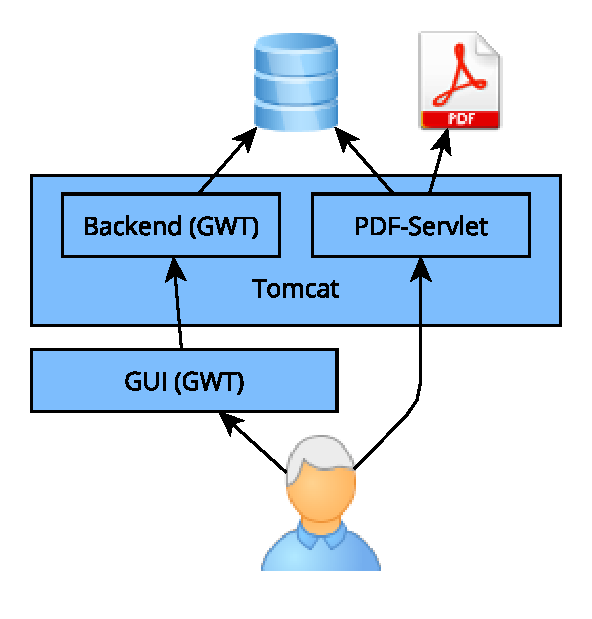
\includegraphics[width=7cm]{images/architektur}
%\end{center}
%\end{frame}


\begin{frame}{Formulare mit \LaTeX: Minihosptiationsbogen}
	\begin{framed}
        \TextField[name=name]{Name} % <--- Formularfeld

	    \hrulefill

    	\begin{center}
        	\Huge
	        Uncool\hspace{0.5em}
    	    $\circ\circ\circ\circ\circ$
        	\hspace{0.5em} Cool
	    \end{center}
    	\smallskip
	\end{framed}
\end{frame}

\begin{frame}[fragile]{Formulare mit \LaTeX: Minihosptiationsbogen}

\begin{minted}{latex}
\begin{framed}
    \begin{Form}
        \TextField[name=name]{Name} % <--- Formularfeld
    \end{Form}

    \hrulefill

    \begin{center}
        \Huge
        Uncool\hspace{0.5em}
        $\circ\circ\circ\circ\circ$
        \hspace{0.5em} Cool
    \end{center}
    \smallskip
\end{framed}
\end{minted}
\end{frame}

\begin{frame}[fragile]{Fomulare mit hyperref}
\framesubtitle{Form}
Alle Felder eines Formulars werden eingeschlossen in
\begin{minted}{latex}
    \begin{Form}[action=http://example.com]
    ...
    \end{Form}
\end{minted}
\begin{itemize}
\item Nur ein \texttt{Form} je Datei
\item Der Optionale Parameter \texttt{action} erlaubt die Formulardaten an eine URL zu senden.
\end{itemize}
\end{frame}


%\begin{frame}[fragile]{Fomulare mit hyperref}
%\framesubtitle{Felder}
%Feldtypen sind
%\begin{Form}[action=http://localhost]
%\begin{itemize}
%	\item \TextField{TextField}
%	\item \CheckBox{CheckBox}
%	\item \ChoiceMenu{ChoiceMenu}{Hans,Peter,Wurst}\\
%	\ChoiceMenu[radio]{ChoiceMenu (Radio)}{Hans,Peter,Wurst}\\
%	\ChoiceMenu[combo]{ChoiceMenu (Combobox)}{Hans,Peter,Wurst}
%	\item \PushButton[onclick={app.alert("Hallo Dante!", 2);}]{PushButton}
%	\item \Submit{Submit}
%	\item \Reset{Reset}
%\end{itemize}
%\end{Form}
%\end{frame}


\begin{frame}[fragile]{Fomulare mit hyperref}
\framesubtitle{Einfache Felder}
\begin{block}{Beispiel}
\begin{itemize}
	\item \TextField[value={42}]{TextField}
	\item \CheckBox[checked]{CheckBox}
\end{itemize}
\end{block}
\begin{block}{Code}
\begin{minted}{latex}
	\TextField[value={42}]{TextField}
	\CheckBox[checked]{CheckBox}
\end{minted}
\end{block}
\begin{block}{Anmerkung}
Mit hyperref erzeugte Checkboxes funktionieren nicht mit allen PDF-Werkzeugen reibungslos: Adobe Acrobat zeigt das \enquote{checked} von hyperref nicht an. iText kann nur Haken entfernen, aber nicht setzen.
\end{block}
\end{frame}


\begin{frame}[fragile]{Fomulare mit hyperref}
\framesubtitle{Choices}
\begin{block}{Beispiel}
\begin{Form}
\begin{itemize}
	\item \ChoiceMenu{ChoiceMenu}{Eins,Zwei,Drei}
	\item \ChoiceMenu[combo]{Combo}{Eins,Zwei,Drei}
	\item \ChoiceMenu[radio]{Radio}{Eins,Zwei,Drei}
\end{itemize}
\end{Form}
\end{block}
\begin{block}{Code}
\begin{minted}{latex}
	\ChoiceMenu{ChoiceMenul}{Eins,Zwei,Drei}
	\ChoiceMenu[combo]{Combo}{Eins,Zwei,Drei}
	\ChoiceMenu[radio]{Radio}{Eins,Zwei,Drei}
\end{minted}
\end{block}
\end{frame}


\begin{frame}[fragile]{Fomulare mit hyperref}
\framesubtitle{Buttons}
\begin{block}{Beispiel}
\begin{Form}[action=http://example.com]
\begin{itemize}
	\item \PushButton[onclick={app.alert("Hallo Dante!", 2);}]{PushButton}
	\item \Submit{Submit}
	\item \Reset{Reset}
\end{itemize}
\end{Form}
\end{block}
\begin{block}{Code}
\begin{minted}{latex}
\PushButton[onclick={app.alert("Hallo Dante!",
    2);}]{PushButton}
\Submit{Submit}
\Reset{Reset}
\end{minted}
\end{block}

%\begin{block}{Anmerkung}
%	\begin{itemize}
%		\item Für umfangreicheres Javascript braucht man Hilfmittel wie insdjs aus dem Acro\TeX-Bundle.
%		\item Je nach PDF-Viewer gibt es JavaScript-APIs.
%	\end{itemize}
%\end{block}
\end{frame}

\begin{frame}[fragile]{Fomulare mit hyperref}
\framesubtitle{Wie funktioniert das Layout (Beispiel)}
Die Kombination aus Label und Textfeld wird so gesetzt:
\begin{minted}{latex}
    \LayoutTextField{#1}{#2}
\end{minted}

Per default \verb|#1 #2|, ergibt also \texttt{Label Feld}.

\end{frame}


\begin{frame}{Ausfüllen mit iText}
iText ist eine freie Programmbibliothek zum Erstellen und Bearbeiten von PDF-Dateien:
\begin{center}
	\url{http://itextpdf.com}
\end{center}
\begin{itemize}
	\item Java, .Net und Android
	\item GNU Affero General Public License (AGPL)
	\item Kommerzielle Lizenz verfügbar.
\end{itemize}
\end{frame}

\begin{frame}[fragile]{Ausfüllen mit iText}
Zurück zu unserem Minibogen:

\bigskip

\begin{minted}{java}
PdfReader reader = new PdfReader("minibogen.pdf");
OutputStream out = new FileOutputStream("out.pdf");

PdfStamper stamper = new PdfStamper(reader, out);
AcroFields form = stamper.getAcroFields();
form.setField("Name", "Hans Wurst");

stamper.close();
reader.close();
\end{minted}
\end{frame}

\begin{frame}[fragile]{Ausfüllen mit iText}
Senden von einer Webanwendung (Servlet):

\bigskip

\begin{minted}{java}
protected void doGet(HttpServletRequest req,
            HttpServletResponse resp) {
    PdfReader reader = new PdfReader("minibogen.pdf");
    OutputStream out = response.getOutputStream();

    response.setContentType("application/pdf");
    PdfStamper stamper = new PdfStamper(reader, out);
    AcroFields form = stamper.getAcroFields();
    form.setField("Name", "Hans Wurst");

    stamper.close();
    reader.close();
}
\end{minted}
\end{frame}


\begin{frame}{Minihospitationsbogen II}
	\begin{framed}
		\begin{Form}
    	    \TextField{Name} % <--- Formularfeld

		    \hrulefill

    		\begin{center}
			    \Huge Uncool\hspace{0.5em}
		    	\large
			    \ChoiceMenu[radio,name=coolness]{}{
			        {}={uncool},
			        {}={fast uncool},
					{}={wer ist das?},
	        		{}={eher cool},
		    	    {}={saucool}
			    }
			    \Huge \hspace{0.5em} Cool
		    \end{center}
    		\smallskip
		\end{Form}
	\end{framed}
\end{frame}


\begin{frame}[fragile]{Minihospitationsbogen II}
Wir erweitern den Bogen:
\begin{minted}{latex}
	\begin{center}
	    \Huge Uncool\hspace{0.5em}
	    \large
	    \ChoiceMenu[radio,name=coolness]{}{
	        {}={uncool},
	        {}={fast uncool},
	        {}={wer ist das?},
	        {}={eher cool},
	        {}={saucool}
	    }
	    \Huge \hspace{0.5em} Cool
	\end{center}
\end{minted}
\end{frame}


\begin{frame}[fragile]{Minihospitationsbogen II}
Und können den Tutor automatisch bewerten ;-)

\begin{minted}{java}
	String field = "coolness";
	String[] states = form.getAppearanceStates(field);
	int evaluation = (int) (Math.random() * states.length);
	form.setField(field, states[evaluation]);
\end{minted}
\end{frame}

\begin{frame}[fragile]{Alternative: PDFtk}

\begin{minted}{bash}
	# Daten via FDF-File
	pdftk form.pdf fill_form data.fdf output form.filled.pdf

	# Daten via STDIN
	pdftk form.pdf fill_form - output form.filled.pdf
\end{minted}

\bigskip

Mehr unter
\begin{center}
	\url{http://www.pdflabs.com/docs/pdftk-man-page/#dest-op-fill-form}
\end{center}

\end{frame}

\begin{frame}{Material im Internet}
\begin{center}
	\url{https://github.com/bitzl/dante-herbsttagung-formulare}
\end{center}
\end{frame}

\begin{frame}[fragile]{Alternativen}
\begin{center}
\Huge
Vielen Dank für die Aufmerksamkeit!

\bigskip

Fragen?
\end{center}

\end{frame}


\end{document}